\documentclass[border=12pt]{standalone}
\usepackage{amssymb}
\usepackage{amsmath}
\usepackage{tikz}
\usetikzlibrary{arrows.meta, decorations.pathreplacing, calc, positioning, shapes.geometric, fit}

% Project palette
\definecolor{cnavy}{HTML}{0E2747}
\definecolor{corange}{HTML}{E8573F}
\definecolor{cgreen}{HTML}{3B9B6D}
\definecolor{cslate}{HTML}{5B6680}
\definecolor{cmuted}{HTML}{9B9484}
\definecolor{ccream}{HTML}{FAFAF6}
\definecolor{cred}{HTML}{B22222}
\definecolor{cblack}{HTML}{1A1A1A}

\begin{document}
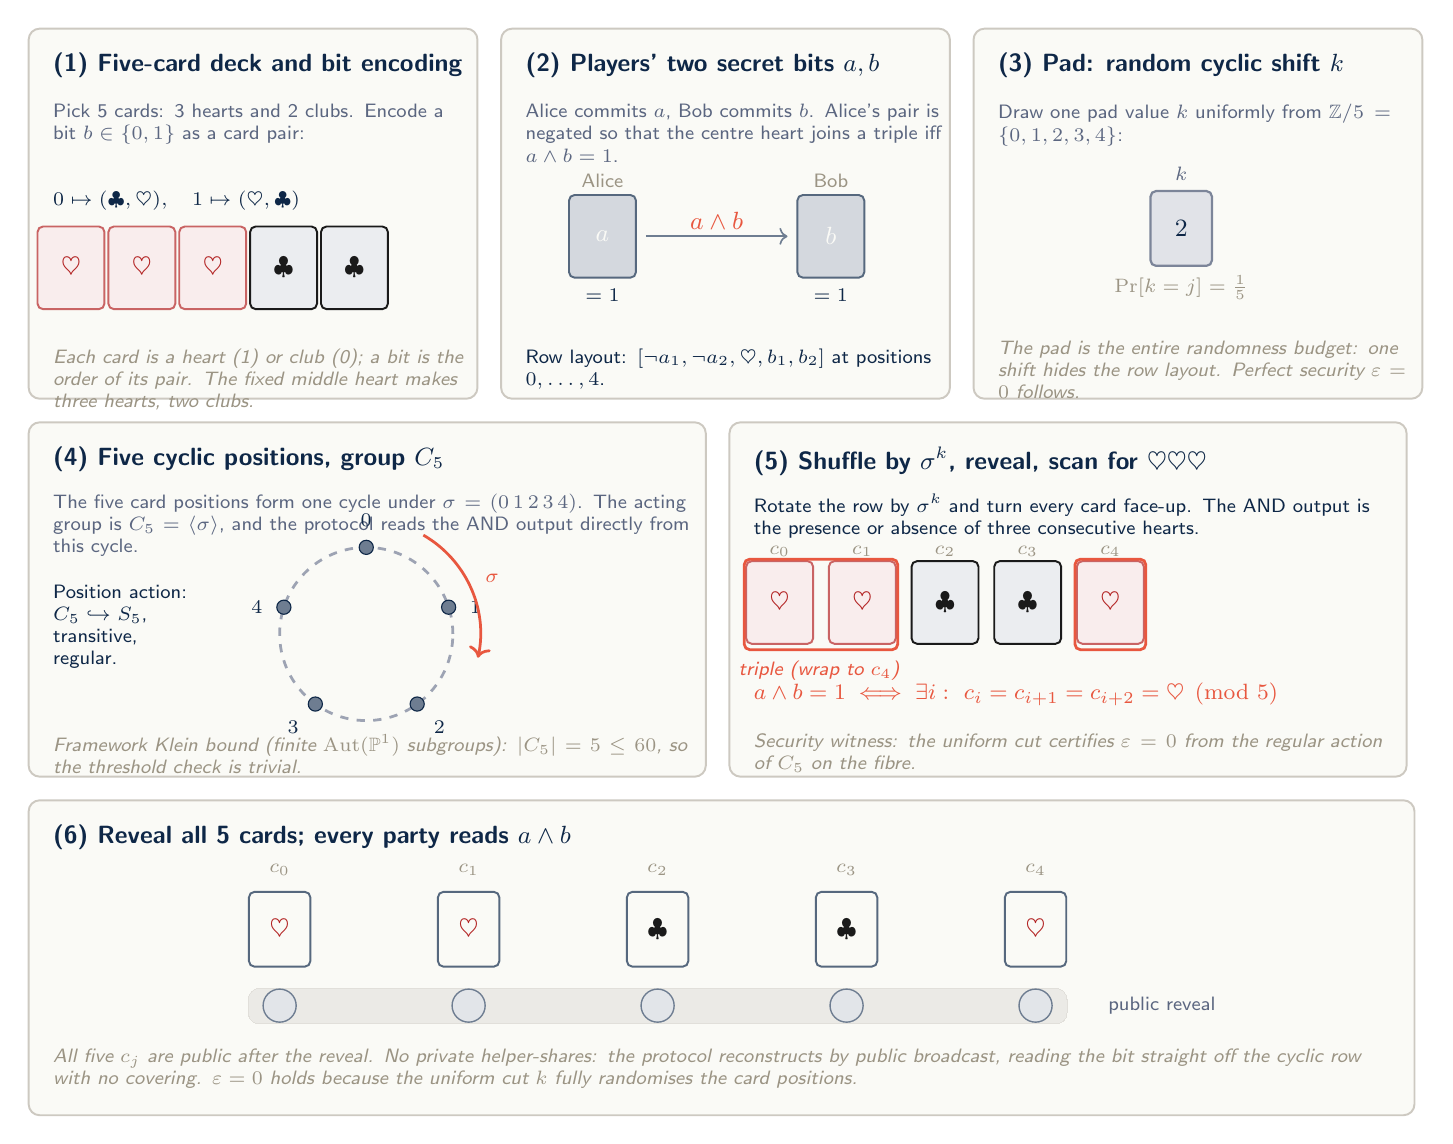
\begin{tikzpicture}[
  panel/.style={
    rectangle, draw=cmuted!50, fill=ccream, rounded corners=4pt,
    line width=0.7pt
  },
  steptitle/.style={cnavy, font=\sffamily\bfseries\small, anchor=north west},
  bodytext/.style={cslate, font=\sffamily\scriptsize, anchor=north west, align=left},
  mathtext/.style={cnavy, font=\sffamily\scriptsize, anchor=north west, align=left},
  redcard/.style={
    rectangle, rounded corners=2pt, draw=cred!70, fill=cred!8,
    line width=0.7pt, minimum width=0.85cm, minimum height=1.05cm,
    inner sep=0pt
  },
  blackcard/.style={
    rectangle, rounded corners=2pt, draw=cblack, fill=cslate!12,
    line width=0.7pt, minimum width=0.85cm, minimum height=1.05cm,
    inner sep=0pt
  },
  facedowncard/.style={
    rectangle, rounded corners=2pt, draw=cnavy!70, fill=cnavy!18,
    line width=0.7pt, minimum width=0.85cm, minimum height=1.05cm,
    inner sep=0pt
  },
  padcard/.style={
    rectangle, rounded corners=2pt, draw=cslate!80, fill=cslate!18,
    line width=0.8pt, minimum width=0.78cm, minimum height=0.95cm,
    inner sep=0pt
  },
  helpercard/.style={
    rectangle, rounded corners=2pt, draw=cnavy!70, fill=ccream,
    line width=0.7pt, minimum width=0.78cm, minimum height=0.95cm,
    inner sep=0pt
  },
  player/.style={
    circle, draw=cnavy!60, fill=cnavy!12, line width=0.5pt,
    minimum size=0.42cm, inner sep=0pt
  },
  font=\sffamily
]

% Canvas layout (top-left at (0, 14)):
%   Row 1 (Steps 1-3): y in [9.0, 14.0],  three panels each 5.7 cm wide
%   Row 2 (Steps 4-5): y in [4.3, 9.0],   two panels each 8.6 cm wide
%   Row 3 (Step 6):    y in [0.0, 4.0],   one full-width panel 17.6 cm

% ============================================================
% Row 1: Steps 1, 2, 3
% ============================================================

% --- Panel 1: Field F_5 and 5-card deck ---
\node[panel, minimum width=5.7cm, minimum height=4.7cm, anchor=north west] (P1)
  at (0.0, 14.0) {};
\node[steptitle] at ($(P1.north west)+(0.20,-0.20)$)
  {(1) Five-card deck and bit encoding};
\node[bodytext, text width=5.3cm]
  at ($(P1.north west)+(0.20,-0.85)$)
  {Pick 5 cards: 3 hearts and 2 clubs. Encode a bit
   $b \in \{0,1\}$ as a card pair:};
\node[mathtext, text width=5.3cm]
  at ($(P1.north west)+(0.20,-1.95)$)
  {$0 \mapsto (\clubsuit,\heartsuit), \quad
    1 \mapsto (\heartsuit,\clubsuit)$};

% Raw deck row (3 hearts + 2 clubs)
\foreach \i/\xp/\suit/\style in {%
  1/0.55/\heartsuit/redcard,
  2/1.45/\heartsuit/redcard,
  3/2.35/\heartsuit/redcard,
  4/3.25/\clubsuit/blackcard,
  5/4.15/\clubsuit/blackcard} {
  \node[\style] at ($(P1.north west)+(\xp, -3.05)$) {};
}
\node[cred, font=\sffamily\bfseries\small] at ($(P1.north west)+(0.55, -3.05)$) {$\heartsuit$};
\node[cred, font=\sffamily\bfseries\small] at ($(P1.north west)+(1.45, -3.05)$) {$\heartsuit$};
\node[cred, font=\sffamily\bfseries\small] at ($(P1.north west)+(2.35, -3.05)$) {$\heartsuit$};
\node[cblack, font=\sffamily\bfseries\small] at ($(P1.north west)+(3.25, -3.05)$) {$\clubsuit$};
\node[cblack, font=\sffamily\bfseries\small] at ($(P1.north west)+(4.15, -3.05)$) {$\clubsuit$};

\node[bodytext, cmuted, font=\sffamily\itshape\scriptsize, text width=5.3cm]
  at ($(P1.north west)+(0.20,-3.95)$)
  {Each card is a heart (1) or club (0); a bit is the order of its pair.
   The fixed middle heart makes three hearts, two clubs.};

% --- Panel 2: Two secret bits a, b ---
\node[panel, minimum width=5.7cm, minimum height=4.7cm, anchor=north west] (P2)
  at (6.0, 14.0) {};
\node[steptitle] at ($(P2.north west)+(0.20,-0.20)$)
  {(2) Players' two secret bits $a, b$};
\node[bodytext, text width=5.3cm]
  at ($(P2.north west)+(0.20,-0.85)$)
  {Alice commits $a$, Bob commits $b$. Alice's pair is negated
   so that the centre heart joins a triple iff $a \wedge b = 1$.};

% Two face-down bit cards
\node[facedowncard] at ($(P2.north west)+(1.30, -2.65)$) {};
\node[ccream, font=\sffamily\bfseries\small] at ($(P2.north west)+(1.30, -2.65)$) {$a$};
\node[cmuted, font=\sffamily\scriptsize] at ($(P2.north west)+(1.30, -1.95)$) {Alice};
\node[cnavy, font=\sffamily\bfseries\scriptsize] at ($(P2.north west)+(1.30, -3.40)$) {$=1$};

\node[facedowncard] at ($(P2.north west)+(4.20, -2.65)$) {};
\node[ccream, font=\sffamily\bfseries\small] at ($(P2.north west)+(4.20, -2.65)$) {$b$};
\node[cmuted, font=\sffamily\scriptsize] at ($(P2.north west)+(4.20, -1.95)$) {Bob};
\node[cnavy, font=\sffamily\bfseries\scriptsize] at ($(P2.north west)+(4.20, -3.40)$) {$=1$};

% Arrow between with AND
\draw[->, cnavy!60, line width=0.6pt]
  ($(P2.north west)+(1.85, -2.65)$) -- ($(P2.north west)+(3.65, -2.65)$);
\node[corange, font=\sffamily\bfseries\small]
  at ($(P2.north west)+(2.75, -2.45)$) {$a \wedge b$};

\node[mathtext, text width=5.3cm]
  at ($(P2.north west)+(0.20,-3.95)$)
  {Row layout: $[\neg a_1,\neg a_2,\heartsuit,b_1,b_2]$
   at positions $0,\dots,4$.};

% --- Panel 3: Pad cyclic shift k ---
\node[panel, minimum width=5.7cm, minimum height=4.7cm, anchor=north west] (P3)
  at (12.0, 14.0) {};
\node[steptitle] at ($(P3.north west)+(0.20,-0.20)$)
  {(3) Pad: random cyclic shift $k$};
\node[bodytext, text width=5.3cm]
  at ($(P3.north west)+(0.20,-0.85)$)
  {Draw one pad value $k$ uniformly from
   $\mathbb{Z}/5 = \{0,1,2,3,4\}$:};

% Single pad card showing k=2
\node[padcard] at ($(P3.north west)+(2.65, -2.55)$) {};
\node[cnavy, font=\sffamily\bfseries\small] at ($(P3.north west)+(2.65, -2.55)$) {$2$};
\node[cslate, font=\sffamily\scriptsize] at ($(P3.north west)+(2.65, -1.85)$) {$k$};

% Tiny labels for the support
\node[cmuted, font=\sffamily\scriptsize] at ($(P3.north west)+(2.65, -3.30)$)
  {$\Pr[k=j]=\tfrac{1}{5}$};

\node[bodytext, cmuted, font=\sffamily\itshape\scriptsize, text width=5.3cm]
  at ($(P3.north west)+(0.20,-3.85)$)
  {The pad is the entire randomness budget: one shift hides the
   row layout. Perfect security $\varepsilon=0$ follows.};

% ============================================================
% Row 2: Steps 4, 5
% ============================================================

% --- Panel 4: Curve P^1/F_5, 5 sheets, trivial monodromy ---
\node[panel, minimum width=8.6cm, minimum height=4.5cm, anchor=north west] (P4)
  at (0.0, 9.0) {};
\node[steptitle] at ($(P4.north west)+(0.20,-0.20)$)
  {(4) Five cyclic positions, group $C_5$};
\node[bodytext, text width=8.2cm]
  at ($(P4.north west)+(0.20,-0.80)$)
  {The five card positions form one cycle under
   $\sigma = (0\,1\,2\,3\,4)$. The acting group is
   $C_5 = \langle \sigma \rangle$, and the protocol reads
   the AND output directly from this cycle.};

% Cycle diagram: 5 positions arranged on a circle, dashed to signal
% "cyclic position set" rather than "algebraic curve".
\draw[cslate!60, line width=1.0pt, dashed]
  ($(P4.north west)+(4.30, -2.70)$) circle (1.10);

% Five points on the circle at angles 90, 90-72, ..., labelled P_0..P_4
\foreach \i/\ang in {0/90, 1/18, 2/-54, 3/-126, 4/162} {
  \node[circle, fill=cnavy!60, draw=cnavy, minimum size=0.18cm, inner sep=0pt]
    (PT\i) at ($(P4.north west)+(4.30, -2.70) + (\ang:1.10)$) {};
}
\node[cnavy, font=\sffamily\scriptsize, anchor=south]
  at ($(PT0.north)+(0,0.05)$) {$0$};
\node[cnavy, font=\sffamily\scriptsize, anchor=west]
  at ($(PT1.east)+(0.05,0)$) {$1$};
\node[cnavy, font=\sffamily\scriptsize, anchor=north west]
  at ($(PT2.south east)+(0.02,-0.02)$) {$2$};
\node[cnavy, font=\sffamily\scriptsize, anchor=north east]
  at ($(PT3.south west)+(-0.02,-0.02)$) {$3$};
\node[cnavy, font=\sffamily\scriptsize, anchor=east]
  at ($(PT4.west)+(-0.05,0)$) {$4$};

% Rotation arrow (orange, outside the circle)
\draw[->, corange, line width=1.0pt]
  ($(P4.north west)+(4.30, -2.70) + (60:1.45)$)
  arc[start angle=60, end angle=-12, radius=1.45];
\node[corange, font=\sffamily\bfseries\scriptsize]
  at ($(P4.north west)+(4.30, -2.70) + (24:1.75)$) {$\sigma$};

% Side note on left
\node[mathtext, text width=2.6cm]
  at ($(P4.north west)+(0.20,-1.95)$)
  {Position action:\\
   $C_5 \hookrightarrow S_5$,\\
   transitive,\\
   regular.};

\node[bodytext, cmuted, font=\sffamily\itshape\scriptsize, text width=8.2cm]
  at ($(P4.north west)+(0.20,-3.85)$)
  {Framework Klein bound (finite $\mathrm{Aut}(\mathbb{P}^1)$ subgroups):
   $|C_5|=5 \le 60$, so the threshold check is trivial.};

% --- Panel 5: Apply sigma^k, reveal, scan ---
\node[panel, minimum width=8.6cm, minimum height=4.5cm, anchor=north west] (P5)
  at (8.9, 9.0) {};
\node[steptitle] at ($(P5.north west)+(0.20,-0.20)$)
  {(5) Shuffle by $\sigma^k$, reveal, scan for $\heartsuit\heartsuit\heartsuit$};
\node[mathtext, text width=8.2cm]
  at ($(P5.north west)+(0.20,-0.80)$)
  {Rotate the row by $\sigma^k$ and turn every card face-up. The AND
   output is the presence or absence of three consecutive hearts.};

% Post-shuffle row for k=2: rot 2 [club,heart,heart,heart,club]
%   = drop 2 ++ take 2 = [heart,heart,club] ++ [club,heart]
%   = [heart, heart, club, club, heart] at positions 0,1,2,3,4
\foreach \i/\xp/\suit/\style/\fg in {%
  0/0.65/\heartsuit/redcard/cred,
  1/1.70/\heartsuit/redcard/cred,
  2/2.75/\clubsuit/blackcard/cblack,
  3/3.80/\clubsuit/blackcard/cblack,
  4/4.85/\heartsuit/redcard/cred} {
  \node[\style] at ($(P5.north west)+(\xp, -2.30)$) {};
  \node[\fg, font=\sffamily\bfseries\small] at ($(P5.north west)+(\xp, -2.30)$) {$\suit$};
  \node[cmuted, font=\sffamily\scriptsize] at ($(P5.north west)+(\xp, -1.65)$) {$c_{\i}$};
}

% Highlight the heart triple at positions {4, 0, 1} (wrap-around)
\draw[corange, line width=1.0pt, rounded corners=2pt]
  ($(P5.north west)+(0.20, -1.75)$) rectangle ($(P5.north west)+(2.15, -2.90)$);
\draw[corange, line width=1.0pt, rounded corners=2pt]
  ($(P5.north west)+(4.40, -1.75)$) rectangle ($(P5.north west)+(5.30, -2.90)$);
\node[corange, font=\sffamily\itshape\scriptsize, anchor=north]
  at ($(P5.north west)+(1.15, -2.92)$) {triple (wrap to $c_4$)};

\node[corange, font=\sffamily\bfseries\footnotesize, anchor=north west]
  at ($(P5.north west)+(0.20,-3.20)$)
  {$a \wedge b = 1 \iff \exists i:\ c_i = c_{i+1} = c_{i+2} = \heartsuit \pmod 5$};

\node[bodytext, cmuted, font=\sffamily\itshape\scriptsize, text width=8.2cm]
  at ($(P5.north west)+(0.20,-3.85)$)
  {Security witness: the uniform cut certifies $\varepsilon=0$ from the
   regular action of $C_5$ on the fibre.};

% ============================================================
% Row 3: Step 6 - distribute 5 revealed cards
% ============================================================

\node[panel, minimum width=17.6cm, minimum height=4.0cm, anchor=north west] (P6)
  at (0.0, 4.2) {};
\node[steptitle] at ($(P6.north west)+(0.20,-0.20)$)
  {(6) Reveal all 5 cards; every party reads $a \wedge b$};

% Five helper-cards spread across the wide panel
% Use same post-shuffle contents: [heart, heart, club, club, heart]
\foreach \j/\xp/\suit/\fg in {%
  0/3.20/\heartsuit/cred,
  1/5.60/\heartsuit/cred,
  2/8.00/\clubsuit/cblack,
  3/10.40/\clubsuit/cblack,
  4/12.80/\heartsuit/cred} {
  \node[helpercard] at ($(P6.north west)+(\xp, -1.65)$) {};
  \node[\fg, font=\sffamily\bfseries\small] at ($(P6.north west)+(\xp, -1.65)$) {$\suit$};
  \node[cmuted, font=\sffamily\scriptsize] at ($(P6.north west)+(\xp, -0.90)$)
    {$c_{\j}$};
}

% Soft band beneath all five player circles to indicate shared observation
\draw[cmuted!30, line width=0pt, fill=cmuted!20, rounded corners=4pt]
  ($(P6.north west)+(2.80, -2.40)$) rectangle ($(P6.north west)+(13.20, -2.85)$);
\foreach \j/\xp in {0/3.20, 1/5.60, 2/8.00, 3/10.40, 4/12.80} {
  \node[player] at ($(P6.north west)+(\xp, -2.62)$) {};
}
\node[cslate, font=\sffamily\scriptsize, anchor=west]
  at ($(P6.north west)+(13.60, -2.62)$) {public reveal};

\node[bodytext, cmuted, font=\sffamily\itshape\scriptsize, text width=17.0cm]
  at ($(P6.north west)+(0.20,-3.05)$)
  {All five $c_j$ are public after the reveal. No private
   helper-shares: the protocol reconstructs by public broadcast, reading the
   bit straight off the cyclic row with no covering. $\varepsilon=0$ holds
   because the uniform cut $k$ fully randomises the card positions.};

\end{tikzpicture}
\end{document}
